% small.tex
\documentclass{beamer}
\usetheme{default}
\usepackage[algo2e]{algorithm2e}
\usepackage{pgf}
\usepackage{tikz}
\usepackage{verbatim}
\usetikzlibrary{arrows,automata}
\usepackage[latin1]{inputenc}

\title{Tools and Algorithms for Deciding Timed Relations}
\subtitle{B Tech Project, 2012-2013}
\author{Mihir Mehta}
\institute{
  Department of Computer Science and Engineering\\
  Indian Institute of Technology, Delhi.\\[1ex]
  \texttt{cs1090197@cse.iitd.ac.in}
}
\date{December 2012}

\begin{document}

\begin{frame}[plain]
  \titlepage
\end{frame}

\begin{frame}{Overview}
  \begin{itemize}
  \item Bisimilarity and related notions
  \item Kanellakis and Smolka's algorithm
  \item Fernandez' algorithm
  \item Paige and Tarjan's algorithm
  \item Timed Automata
  \item Equivalences on Timed Automata
  \item Code written so far
  \end{itemize}
\end{frame}

\begin{frame}{Bisimilarity and related notions}
  \begin{itemize}
  \item Labeled Transition System: This is a triple $(Proc,Act,\{
    \xrightarrow{a} | a \epsilon Act \})$ where
    \begin{itemize}
    \item $Proc$ is a set of states (also called processes or
      configurations.)
    \item $Act$ is a set of actions (also called labels.)
    \item $\xrightarrow{a} \subseteq Proc \times Proc$ is a transition relation.
    \end{itemize}
  \item CCS expression: Defined by the following grammar:
    \begin{itemize}
    \item $P::=K$
    \item $P::=\alpha . P$
    \item $P::=_{i \epsilon I} P_i$
    \item $P::=P|Q$
    \item $P::=P[f]$
    \item $P::=P\L$
    \end{itemize}
  \end{itemize}
\end{frame}

\begin{frame}{Bisimilarity and related notions}
  \begin{itemize}
  \item Equivalence for CCS
    processes.
  \item Trace equivalence: $Traces(P) = Traces(Q)$
  \item Unsatisfactory (differences in deadlock
    behaviour.)
  \item Strong bisimulation: A binary relation $R$ is a \textit{strong
    bisimulation} if and only if, for all $(s_1, s_2) \epsilon R$ and $a \epsilon Act .$\\
    $\forall s_1' (s_1 \xrightarrow{a} s_1' \Rightarrow \exists s_2'
    . (s_2 \xrightarrow{a} s_2' \wedge (s_1', s_2') \epsilon R ) )
    \wedge $ \\
    $\forall s_2' (s_2 \xrightarrow{a} s_2' \Rightarrow \exists s_1'
    . (s_1 \xrightarrow{a} s_1' \wedge (s_1', s_2') \epsilon R ) )$
  \item It can be shown that the union of all strong bisimulations
    over the set of states is a strong bisimulation. This binary
    relation is called \textit{strong bisimilarity}, denoted by $\sim$.
  \end{itemize}
\end{frame}

\begin{frame}{Bisimilarity and related notions}
  \begin{itemize}
  \item Better notion of equivalence than trace
    equivalence: picks up differences in the deadlock
    behaviour of processes under study.
  \item Failing: does not account for the
    invisible nature of $\tau$ transitions in CCS processes.
  \item Weak bisimulation: A binary relation $R$ is a \textit{weak
    bisimulation} if and only if, for all $(s_1, s_2) \epsilon R$ and $a \epsilon Act .$\\
    $\forall s_1' (s_1 \xrightarrow{a} s_1' \Rightarrow \exists s_2'
    . (s_2 \overset{a}{\Rightarrow} s_2' \wedge (s_1', s_2') \epsilon R ) )
    \wedge $ \\
    $\forall s_2' (s_2 \xrightarrow{a} s_2' \Rightarrow \exists s_1'
    . (s_1 \overset{a}{\Rightarrow} s_1' \wedge (s_1', s_2') \epsilon R ) )$
  \item It can be shown that the union of all weak bisimulations
    over the set of states is a weak bisimulation. This binary
    relation is called \textit{weak bisimilarity}, denoted by $\approx$.
  \item Better suited to CCS processes,
    as it ignores $\tau$ transitions, thus disregarding hidden
    behaviour within a process.
  \end{itemize}
\end{frame}

\begin{frame}{Kanellakis and Smolka's algorithm}
  \begin{itemize}
  \item This is a naive algorithm for determining the bisimilarity
    relation for the set of processes in a labelled transition system.
  \item This relies on the notion of a splitter.
  \item Let $\pi = \{ B_0, ..., B_k \}, k \ge 0$ be a partition of the
    set of states $Pr$ in a labeled transition system.
  \item A splitter for a block $B_i$ $\epsilon$ $\pi$ is a block $B_j$
    $\epsilon$ $\pi$ such that for some action $a$ $\epsilon$ $Act$, some
    states in $B_i$ have $a$-labelled transitions whose targets lie in
    $B_j$ while other states in $B_i$ do not.
  \item This suggests a refinement of $\pi$: replace block $B_i$ with
    \\
    $B_i^1 = B_i \cap T_a^{-1}[B_j] $ \\
    $B_i^2 = B_i - B_i^1 $
  \item Refinements of this kind constitute the steps of this
    algorithm.
  \end{itemize}
\end{frame}

\begin{frame}[fragile]

  \frametitle{Kanellakis and Smolka's algorithm}

  \begin{algorithm2e}[H]
    Initialise $\pi$ to ${Pr}$\;
    \While{there exist splitters among the elements of $\pi$}{
      Pick a splitter $B$\;
      \ForEach {$B_j$ $\epsilon$ $\pi$} {
        \ForEach{$a$ $\epsilon$ $Act$}{
          Split $B_j$ with respect to $B$ for
          action $a$\;
        }
      }
    }
    Return $\pi$\;
\end{algorithm2e}

  \begin{itemize}
  \item The time complexity of this algorithm is $O(mn)$, since there
    can be at most n iterations, and all m edges are scanned in each iteration.
  \end{itemize}

\end{frame}

%% \begin{frame}{Kanellakis and Smolka's algorithm}
%%   \begin{tikzpicture}[->,>=stealth',shorten >=1pt,auto,node
%%       distance=2.8cm,
%%       semithick]
%%     \tikzstyle{every state}=[fill=red,draw=none,text=white]

%%     \node[initial,state] (A)                    {$q_0$};
%%     \node[state]         (B) [below right of=A] {$q_1$};
%%     \node[state]         (C) [below of=B] {$q_2$};
%%     \node[state]         (D) [below left of=C] {$q_3$};
%%     \node[state]         (E) [above left of=D]       {$q_4$};
%%     \node[state]         (F) [above of=E]       {$q_5$};

%%     \path (A) edge              node{a} (B)
%%     edge              node{b} (D)
%%     (B) edge node{a} (C)
%%     edge              node{b} (D)
%%     edge              node{b} (E)
%%     (C) edge              node{a} (B)
%%     edge node{b}  (E)
%%     (D) edge node{c} (F)
%%     (E) edge node{c} (F);
%%   \end{tikzpicture}
%% \end{frame}

%% \begin{frame}{Kanellakis and Smolka's algorithm}
%%   \begin{tikzpicture}[->,>=stealth',shorten >=1pt,auto,node
%%       distance=2.8cm,
%%       semithick]
%%     \tikzstyle{every state}=[fill=blue,draw=none,text=white]

%%     \node[initial,state] (A)                    {$q_0$};
%%     \node[state]         (B) [below right of=A] {$q_1$};
%%     \node[state]         (C) [below of=B] {$q_2$};
%%     \tikzstyle{every state}=[fill=red,draw=none,text=white]

%%     \node[state]         (D) [below left of=C] {$q_3$};
%%     \node[state]         (E) [above left of=D]       {$q_4$};
%%     \node[state]         (F) [above of=E]       {$q_5$};

%%     \path (A) edge              node{a} (B)
%%     edge              node{b} (D)
%%     (B) edge node{a} (C)
%%     edge              node{b} (D)
%%     edge              node{b} (E)
%%     (C) edge              node{a} (B)
%%     edge node{b}  (E)
%%     (D) edge node{c} (F)
%%     (E) edge node{c} (F);
%%   \end{tikzpicture}
%% \end{frame}

%% \begin{frame}{Kanellakis and Smolka's algorithm}
%%   \begin{tikzpicture}[->,>=stealth',shorten >=1pt,auto,node
%%       distance=2.8cm,
%%       semithick]
%%     \tikzstyle{every state}=[fill=blue,draw=none,text=white]

%%     \node[initial,state] (A)                    {$q_0$};
%%     \node[state]         (B) [below right of=A] {$q_1$};
%%     \node[state]         (C) [below of=B] {$q_2$};
%%     \tikzstyle{every state}=[fill=yellow,draw=none,text=white]

%%     \node[state]         (D) [below left of=C] {$q_3$};
%%     \node[state]         (E) [above left of=D]       {$q_4$};
%%     \tikzstyle{every state}=[fill=red,draw=none,text=white]

%%     \node[state]         (F) [above of=E]       {$q_5$};

%%     \path (A) edge              node{a} (B)
%%     edge              node{b} (D)
%%     (B) edge node{a} (C)
%%     edge              node{b} (D)
%%     edge              node{b} (E)
%%     (C) edge              node{a} (B)
%%     edge node{b}  (E)
%%     (D) edge node{c} (F)
%%     (E) edge node{c} (F);
%%   \end{tikzpicture}
%% \end{frame}

\begin{frame}{Fernandez' algorithm}
  \begin{itemize}
  \item More efficient algorithm (O(m log n)).
  \item Relies on Paige and Tarjan's technique of three-way splitting.
  \item Splitters can now be 'simple' or 'compound'.
  \item Stability: A partition $\pi$ is said to be stable with respect to a
    compound block S if S is not a splitter for any block in $\pi$ for
    any action.
  \item For a compound block S, having a constituent simple block B
    satisfying $n(B) \le 0.5*n(S)$, and with respect to which $\pi$ is
    stable, we can split a block $B_i$ on an action $a$ as follows:\\
    $B_i^1 = (B_i \cap T_a^{-1}[B]) - T_a^{-1}[S-B]$ \\
    $B_i^2 = (B_i \cap T_a^{-1}[S-B]) - T_a^{-1}[B]$ \\
    $B_i^3 = B_i \cap T_a^{-1}[B] \cap T_a^{-1}[S-B]$ \\
  \end{itemize}
\end{frame}

\begin{frame}[fragile]

  \frametitle{Fernandez' algorithm}
  \begin{algorithm2e}[H]
    Initialise $\pi = \{Pr\}$\;
    Initialise W = $\{Pr\}$
    \While{W is not empty}{
      Choose a splitter B from W, removing it\;
      \eIf{B is a simple splitter}{
        Perform a two-way split on each action with respect to B and
        update W\;
      }{
        Perform a three-way split on each action with respect to B and
        update W\;
      }
    }
  \end{algorithm2e}
\end{frame}

\begin{frame}{Paige and Tarjan's Algorithm}
  \begin{itemize}
  \item Technique of three way splitting came from here.
  \item Special case of Fernandez' algorithm when there's only one
    kind of action.
  \end{itemize}
\end{frame}

\begin{frame}{Timed Automata}
  \begin{itemize}
  \item Formally, a timed automaton over a finite set of clocks $C$
    and a finite set of actions $Act$ is a 4-tuple $(L, l_{0}, E, I)$.
  \item $L$ is a finite set of locations.
  \item $l_{0}$ is the initial location.
  \item $E \subseteq L \times B(C) \times Act \times 2^{C} \times L$
    is a finite set of edges.
  \item $I: L \rightarrow B(C)$ assigns invariants to each edge
    location.
  \item $B(C)$ is the set of clock constraints over C. An element of $B(C)$
    can be an equality, a slack inequality, a strict inequality, or
    an AND combination of such constraints.
  \end{itemize}
\end{frame}

\begin{frame}{Equivalences on Timed Automata}

  \begin{itemize}
  \item \emph{Timed bisimulation}: A binary relation $R$ is a timed
    bisimulation if and only if, for all $(s_1, s_2) \epsilon R$ , $a \epsilon Act $, $d \epsilon R_{\ge 0}$\\
    $\forall s_1' (s_1 \xrightarrow{a} s_1' \Rightarrow \exists s_2'
    . (s_2 \xrightarrow{a} s_2' \wedge (s_1', s_2') \epsilon R ) )
    \wedge $ \\
    $\forall s_2' (s_2 \xrightarrow{a} s_2' \Rightarrow \exists s_1'
    . (s_1 \xrightarrow{a} s_1' \wedge (s_1', s_2') \epsilon R ) ) \wedge $ \\
    $\forall s_1' (s_1 \xrightarrow{d} s_1' \Rightarrow \exists s_2'
    . (s_2 \xrightarrow{d} s_2' \wedge (s_1', s_2') \epsilon R ) )
    \wedge $ \\
    $\forall s_2' (s_2 \xrightarrow{d} s_2' \Rightarrow \exists s_1'
    . (s_1 \xrightarrow{d} s_1' \wedge (s_1', s_2') \epsilon R ) ) $ \\

  \item It can be shown that the union of all timed bisimulations
    over the set of (location, valuation) pairs is a timed bisimulation. This binary
    relation is called \textit{timed bisimilarity}, denoted by $\sim$.
  \end{itemize}

\end{frame}

\begin{frame}{Equivalences on Timed Automata}

  \begin{itemize}
  \item \emph{Time abstracted bisimulation}: A binary relation $R$ is
    a time abstracted
    bisimulation if and only if, for all $(s_1, s_2) \epsilon R$ , $a \epsilon Act $, $d \epsilon R_{\ge 0}$\\
    $\forall s_1' (s_1 \xrightarrow{a} s_1' \Rightarrow \exists s_2'
    . (s_2 \xrightarrow{a} s_2' \wedge (s_1', s_2') \epsilon R ) )
    \wedge $ \\
    $\forall s_2' (s_2 \xrightarrow{a} s_2' \Rightarrow \exists s_1'
    . (s_1 \xrightarrow{a} s_1' \wedge (s_1', s_2') \epsilon R ) ) \wedge $ \\
    $\forall s_1' (s_1 \xrightarrow{d} s_1' \Rightarrow \exists (s_2',
    d')
    . (s_2 \xrightarrow{d'} s_2' \wedge (s_1', s_2') \epsilon R ) )
    \wedge $ \\
    $\forall s_2' (s_2 \xrightarrow{d} s_2' \Rightarrow \exists (s_1', d')
    . (s_1 \xrightarrow{d'} s_1' \wedge (s_1', s_2') \epsilon R ) ) $ \\

  \item It can be shown that the union of all time abstracted bisimulations
    over the set of (location, valuation) pairs is a time abstracted
    bisimulation. This binary
    relation is called \textit{time abstracted bisimilarity}, denoted
    by $\sim_u$.
  \end{itemize}

\end{frame}

\begin{frame}{Equivalences on Timed Automata}

  \begin{itemize}

  \item \emph{Equivalence of valuations}: Two valuations $v$ and $v'$ of
    a timed automaton are said to be equivalent ($v \equiv v'$) if and
    only if:
    \begin{itemize}
    \item For each $x$ $\epsilon$ $C$, either both $v(x)$ and $v'(x)$ are
      greater than $c_x$ or $\lfloor v(x) \rfloor = \lfloor v'(x)
      \rfloor$
    \item For each $x$ $\epsilon$ $C$ such that $v(x) \le c_x$,
      $frac(v(x))=0$ if and only if $frac(v'(x))=0$.
    \item For all $x,y$ $\epsilon$ $C$ such that $v(x) \le c_x$ and $v(y)
      \le c_y$, we have $frac(v(x)) \le frac(v(y))$ if and only if
      $frac(v'(x)) \le frac(v'(y))$.
    \end{itemize}

  \item Under this notion of equivalence, an equivalence class is known
    as a \emph{region}. The equivalence class containing a valuation $v$
    is denoted by $[v]_{\equiv}$.

  \end{itemize}

\end{frame}

\begin{frame}{Timed equivalences example}

  \begin{tikzpicture}[->,>=stealth',shorten >=1pt,auto,node
      distance=2.8cm,
      semithick]
    \tikzstyle{every state}=[fill=red,draw=none,text=white]
    
    \node[initial,state] (A)              {$A$};
    \node[state]         (B) [below of=A] {$B$};
    \node[initial,state] (C) [right of=A] {$A'$};
    \node[state]         (B) [below of=C] {$B'$};
    
    \path (A) edge              node {$x \le 1$\\$a$\\$x:=0$}    (B)
    (C) edge              node {$x \le 2$\\$a$\\$x:=0$}    (D);
  \end{tikzpicture}

\end{frame}

\begin{frame}{Equivalences on Timed Automata}

  \begin{itemize}

  \item \emph{Region graph}: the region graph of a timed automaton $A$ with clock set $C$
    and action set $Act$ is an LTS\\
    $T_r(A) = (Proc,Act \cup \{\varepsilon\}, \{\xrightarrow{a}|a \epsilon
    Act \cup \{\varepsilon\}\})$\\
    where $Proc = \{(l, [v]_{\equiv}) | l \epsilon L, v: C \rightarrow
    R_{\ge 0}\}$ (these states are called symbolic states)\\
    The transitions are defined as follows:
    \begin{itemize}
    \item For each $a \epsilon A$, $(l, [v]_{\equiv})
      \overset{a}{\Rightarrow} (l', [v']_{\equiv})$ iff $(l,v)
      \overset{a}{\rightarrow} (l', v')$
    \item $(l, [v]_{\equiv}) \xrightarrow{a} (l, [v']_{\equiv})$ if
      for some $d \epsilon R_{\ge 0}$, $(l, v) \xrightarrow{d} (l,
      v')$
    \end{itemize}

  \end{itemize}

\end{frame}

\begin{frame}{Equivalences on Timed Automata}

  \begin{itemize}

    \item \emph{Extended Clock Constraints}: These are described by the  grammar\\
    $g :: = x \bowtie n | x - y \bowtie n | g_1 \wedge g_2$\\

    \item The set of extended clock constraints is denoted by $B^+(C)$

    \item \emph{Zones}: A zone is a set of valuations represented by an
      extended clock constraint.\\
      $Z = {v|v \epsilon g_Z}$

    \item \emph{Symbolic state}: For a timed automaton $A$, a symbolic
      state is an ordered pair of a location and a zone, that is, $(l,
      Z)$.

  \end{itemize}

\end{frame}

\begin{frame}{Equivalences on Timed Automata}

  \begin{itemize}

    \item \emph{Reachability graph}: The reachability graph of a timed
      automaton is a directed graph in which the nodes are symbolic states
      and the edges are given by the \emph{reachability relation}:
      \begin{itemize}
      \item $(l,Z')$ is reachable from $(l,Z)$ if there exists a
        valuation belonging $Z'$ which can be obtained
        from Z by applying a time delay which does not violate the
        invariant at $l$.

      \item $(l', Z')$ is reachable from $(l, Z)$ if $l$ has an action
        transition to $l'$ and there exists a valuation in $Z'$ which
        violates neither the guard of the
        transition nor the invariant at $l'$ after performing the
        clock resets required by the transition.

      \end{itemize}

  \end{itemize}

\end{frame}

\begin{frame}{Code written so far}

  \begin{itemize}

    \item \emph{Fernandez' algorithm}: We expect to need this
      algorithm while building the software, so we built a module
      implementing it in Ocaml (primary language for this project.)

    \item \emph{Grammar}: We implemented a lexer and parser in Ocaml
      to build a representation of a timed automaton from a
      specification in a text file.

  \end{itemize}

\end{frame}

\begin{frame}{Timed automaton example}

\begin{verbatim}

#states 3
#trans 6
#clocks 1
X

state: 0
invar: TRUE
trans:
TRUE => RESET { X }; goto 1

state: 1
invar: TRUE
trans:
X <= 2 => RESET {  }; goto 0
X > 2 => RESET {  }; goto 2

state: 2
invar: TRUE
trans:
TRUE => RESET {  }; goto 0

\end{verbatim}

\end{frame}

\begin{frame}{Timed automaton example}

  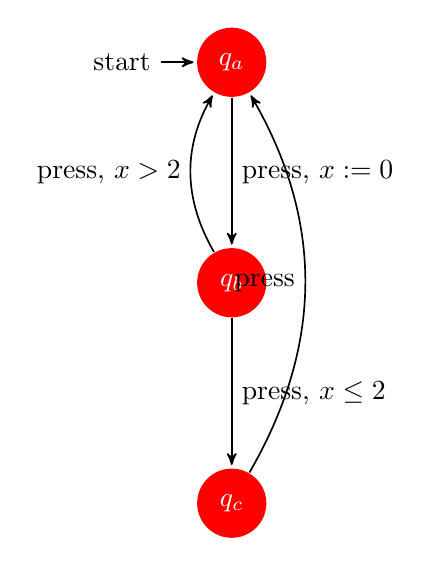
\begin{tikzpicture}[->,>=stealth',shorten >=1pt,auto,node
      distance=2.8cm,
      semithick]
    \tikzstyle{every state}=[fill=red,draw=none,text=white]
    
    \node[initial,state] (A)                    {$q_a$};
    \node[state]         (B) [below of=A] {$q_b$};
    \node[state]         (C) [below of=B] {$q_c$};
    
    \path (A) edge              node {press, $x:=0$}    (B)
    (B) edge [bend left] node {press, $x > 2$}        (A)
    edge              node {press, $x \le 2$}         (C)
    (C) edge [bend right] node {press}                  (A);
  \end{tikzpicture}
  
\end{frame}

\begin{frame}{References}

\begin{itemize}
\item Reactive Systems: Modeling, Specification and Verification -
  Luca Aceto, Anna Ingolfsdottir, Kim Larsen, Jiri Srba.
\end{itemize}

\end{frame}

\end{document}
